% !TEX encoding = UTF-8 Unicode
\documentclass[10pt, a4paper]{article}

\usepackage{amsmath}
\usepackage{footnote}
\makesavenoteenv{tabular}
\usepackage{ltc05}
%\usepackage{polski}
\usepackage[utf8]{inputenc}
\usepackage{textcomp} 
\usepackage[T1]{fontenc}
\usepackage{lmodern}
\usepackage{url}
\usepackage{graphicx}
\title{A Sequential Child Combination Tree-LSTM Network for Sentiment Analysis}


%%%%%%%%%%%%%%%%%%%%%%%%%%%%%%%%%%%%%%%%%%%%%%%%%%%%%%%%%%%%%%%%%%%%%%%%%
%!!!!!!!!!!!!!!!!!!!!!!!!!!!!!!!!!!!!!!!!!!!!!!!!!!!!!!!!!!!!!!!!!!!!!!!!
%!!!!!!!!!!!!!!!!!!!!!!!!!!!!!!!!!!!!!!!!!!!!!!!!!!!!!!!!!!!!!!!!!!!!!!!!
% PLEASE DO NOT WRITE YOUR NAME AND ADDRESS IN THE DRAFT OF YOUR PAPER
% SIMPLY ERASE THE LINES...
\name{ML$^{\dagger}$\\ \bf \large PęP$^{\ast}$} 

\address{ $^{\dagger}$VoiceLab \\	
               michal.lew@voicelab.pl \\ \\
               $^{\ast}$University of Lodz \\ 
               piotr.pezik@uni.lodz.pl}

%% ... UP TO HERE
% ... UP TO HERE
%!!!!!!!!!!!!!!!!!!!!!!!!!!!!!!!!!!!!!!!!!!!!!!!!!!!!!!!!!!!!!!!!!!!!!!!!
%!!!!!!!!!!!!!!!!!!!!!!!!!!!!!!!!!!!!!!!!!!!!!!!!!!!!!!!!!!!!!!!!!!!!!!!!
%%%%%%%%%%%%%%%%%%%%%%%%%%%%%%%%%%%%%%%%%%%%%%%%%%%%%%%%%%%%%%%%%%%%%%%%%


\abstract{This paper evaluates thsdfh.}

\begin{document}

\maketitleabstract

\section{Introduction}   
Sentiment Analysis (SA) is an active area of natural language processing research with applications in general opinion mining, customer relations management systems, marketing and social media communication studies to mention just a few examples. A common objective of SA is to automatically detect the attitudinal value of an utterance or otherwise coherent stretch of text which can be attributed to a particular author. The distribution of  such attitudinal values in an utterance is usually known as its \textit{polarity} and it usually ranges from positive to neutral and negative \cite{cambria_schuller}, possibly with finer-grained distinctions between these main categories, such as \textit{somewhat positive} or \textit{very negative} \cite{socher2013recursive}. More recent approaches to SA focus on phrase-level polarity classification, whereby attitudinal or emotional values are detected at the level of syntactic phrases and only then compositionally combined to compute the polarity of an entire utterance. Such approaches are particularly important in aspect-based SA, where different aspects of one's opinion about a product, movie, person, etc. have to be detected in addition to  classifying the overall sentiment of a text unit. Also, phrase-level SA is better suited to deal with basic syntactic phenomena such as negation or modality which may cause a significant shift in the predominant sentiment of an utterance \cite{wilson_wiebe}. For example, the overall polarity of the Polish sentence shown in Table \ref{tab:nie_drazni_1}, which describes a buyer's overall satisfaction with a particular brand of perfume, is positive, even though its (directly negated) main verb \textit{drażnić} (irritate) could be found in a list of keywords denoting negative sentiment. 
\par The present paper evaluates a deep-learning based system for syntax-driven SA, which was submitted to the PolEval 2017 competition. We first briefly describe the syntactically annotated sentiment datasets used and the nature of the classification task. Next, we present the Sequential Child-Combination Tree-LSTM Network model used to implement the proposed system and evaluate its performance on the PolEval test set.


\section{PolEval 2017}

The dataset released in the PolEval competition for the task described in this paper can be described as a sentiment dependency treebank. In general, sentiment treebanks are syntactically-parsed collections of sentiment-annotated sentences. For example, the Stanford Sentiment Treebank \cite{socher2013recursive}
 
which could be translated word-for-word into English as \textit{(It) doesn't irritate even after a whole day.}

\begin{table}[h]
 \begin{center}
\begin{tabular}{|l| l l l l l l l|}
      \hline
      %Level&Tools\\
      %\hline\hline
      W & Nie & drażni & nawet & po & całym & dniu & . \\
      \hline
      P & 2 & 0 & 2 & 2 & 6 & 4 & 2 \\
      \hline
      S & 0 & 1 & 0 & 0 & 0 & 0 & 0 \\
      \hline
\end{tabular}
\caption{An example PolEval dataset sentence with phrase-level sentiment annotation (W -- word nodes, P -- syntactic parents, S -- polarity value).}
\label{tab:nie_drazni_1}
 \end{center}
\end{table}



\begin{figure}
  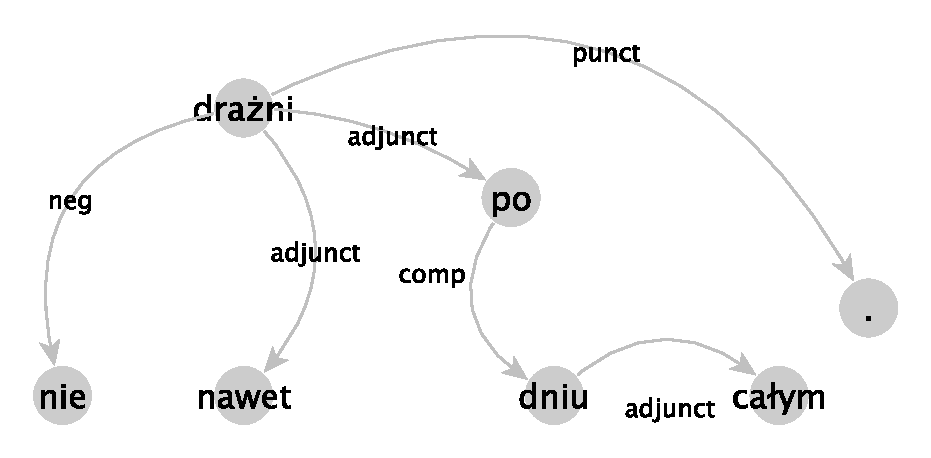
\includegraphics[width=\linewidth]{imgs/nie_drazni.pdf}
  \caption{A dependency representation of the example sentence shown in Table \ref{tab:nie_drazni_1}.}
  \label{fig:boat1}
\end{figure}

\begin{table}[h]
 \begin{center}
\begin{tabular}{|l | l|}

\hline
 Word &	Polarity\\
      \hline
     Nie &	0\\
     \hline
Nie drażni nawet po całym dniu	 . & 1\\
\hline
nawet &	0\\
\hline
po całym dniu &	0\\
\hline
całym dniu &	0\\
\hline
.	& 0\\
      \hline
\end{tabular}
\caption{Phrase- and word-level sentiment values to be predicted for the example sentence shown in Table \ref{tab:nie_drazni_1}.}
\label{tab:nie_drazni_2}
 \end{center}
\end{table}






\section{Model} 


\subsection{LSTM}

Recurrent Neural Networks have been widely used for many task in natural language processing. They can process the arbitrary long inputs by recurrent application of transition function over hidden state. 
	The most common form of RNN's transition function is an affine transformation followed by hyperbolic tangent function
	\begin{equation} h_t = tanh(W_{x_t}+U_{h_{t-1}}+b)
\end{equation}
	  	This gives them ability to use the information gathered in previous states when processing text. In theory it makes them able to look at the infinite history while processing sequences of words. 	Unfortunately they suffer from so called vanishing gradient problem, which means that during training gradient can grow or decay exponentially over long sequences [s (Hochreiter,
1998; Bengio et al., 1994)]
	The LSTM architecture (Hochreiter and Schmidhuber, 1997) addresses this problem of learning long-term dependencies by introducing a memory cell that is able to preserve state over long periods of time. [citation]
		There are many different variants of LSTMs, in our work we used following equations:
		
\begin{equation}
\begin{split}
		&i_t = \sigma(U_{x_t}^i + W_{s_t-1}^i + b^i) ,\\
		&f_t = \sigma(U_{x_t}^f + W_{s_t-1}^f + b^f) ,\\
		&o_t = \sigma(U_{x_t}^o + W_{s_t-1}^o + b^o) ,\\
		&g_t = \tanh(U_{x_t}^g+ W_{s_t-1}^g + b^g) ,\\
		&c_t = c_{t-1} \bullet f_t + g_t \bullet i_t ,\\
		&s_t = \tanh(c_t) \bullet o_t 
\end{split}
\end{equation}

		where $x_t$ is input at current time step, $i_t$ is an input gate, $f_t$ a forget gate, $o_t$ an output gate and $c$ stands for LSTM memory.
		The gates mechanism controls how much information from past states and memory is used at the current time step. 

\subsection{Tree-LSTM}
	The problem with classical LSTM's is that they are linear chain which makes them useless for processing more sophisticated structures than sequences. In particular, many linguistic beings are represented with tree-structure [citation?].
	In order to process tree-structured data we need to extend the LSTM architecture. In our work we propose Sequential Child-Combination Tree-LSTM.
	In general, tree-structured Recurrent Neural Networks expand basic RNNs by creating a way to plug in more than one previous state to hidden unit at current time step.
	[obrazek podłączanie 2 poprzednich stanów do nowego]
	The essence lie in the way in which the children states are combined with parent state.

\subsection{Child-Sum Tree-LSTM}
Child-Sum Tree-LSTM equations

	
\subsection{Sequential-Child-Combination Tree-LSTM}

\begin{figure}[h]
	 \begin{center}
    	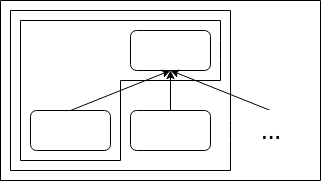
\includegraphics[width=0.5\textwidth]{sequentialchild}
		\caption{Sequentially combining the children with parent}
	 \end{center}
\end{figure}
	In our work we combine children with its parent as follows:
\begin{equation}
\begin{split}
&i_{ch_1} = \sigma(U_{x_t}^i + W_{s_{t-1}}^i + b^i) ,\\
&f_{ch_1} = \sigma(U_{x_t}^f + W_{s_{t-1}}^f + b^f) ,\\
&o_{ch_1} = \sigma(U_{x_t}^o + W_{s_{t-1}}^o + b^o) ,\\
&g_{ch_1} = \tanh(U_{x_t}^g+ W_{s_{t-1}}^g + b^g) ,\\
&c_{ch_1} = c_{t-1} \bullet f_{ch_1} + g_{ch_1} \bullet i_{ch_1} ,\\
&s_{ch_1} = \tanh({c_{ch_1}}) \bullet o_{ch_1},\\\\
&i_{ch_2} = \sigma(U_{x_t}^i + W_{ch_1}^i + b^i) ,\\
&f_{ch_2} = \sigma(U_{x_t}^f + W_{ch_1}^f + b^f) ,\\
&o_{ch_2} = \sigma(U_{x_t}^o + W_{ch_1}^o + b^o) ,\\
&g_{ch_2} = \tanh(U_{x_t}^g+ W_{ch_1}^g + b^g) ,\\
&c_{ch_2} = c_{ch_1} \bullet f_{ch_2} + g_{ch_2} \bullet i_{ch_2} ,\\
&s_{ch_2} = \tanh(c_{ch_2}) \bullet o_{ch_2},\\\\
&\cdots\\\\
&i_{ch_n} = \sigma(U_{x_t}^i + W_{ch_{n-1}}^i + b^i) ,\\
&f_{ch_n} = \sigma(U_{x_t}^f + W_{ch_{n-1}}^f + b^f) ,\\
&o_{ch_n} = \sigma(U_{x_t}^o + W_{ch_{n-1}}^o + b^o) ,\\
&g_{ch_n} = \tanh(U_{x_t}^g+ W_{ch_{n-1}}^g + b^g) ,\\
&c_{ch_n} = c_{ch_n} \bullet f_{ch_n} + g_{ch_n} \bullet i_{ch_n} ,\\
&s_{ch_n} = \tanh(c_{ch_n}) \bullet o_{ch_n},\\\\
&s_{t} = s_{ch_n}
\end{split}
\end{equation}
	where $s_{ch_i}$ is an intermediate state after combining with i-th children.\\
Intuicyjnie, łączymy dzieci z rodzicem od lewej do prawej w taki sposób, że tworzymy pośrednie zanurzenia niosące informację o ojcu uzupełnioną o informację o poddrzewie, którego korzeniem jest dane dziecko.
Ostateczny stan po połączeniu ze wszystkimi dziećmi tworzy znaczenie całego drzewa.
Przykład 'Stary rudy kot wlazł na płot'
mamy kot-stary kot-rudy kot-wlazł
z tego wychodzi, że stary kot-rudy stary kot-wlazł
stary rudy kot-wlazł itd.
można przedstawić taki przykład, żeby pokazać intuicję stojącą za tym sposobem.
\begin{figure}[h]
	\begin{center}
		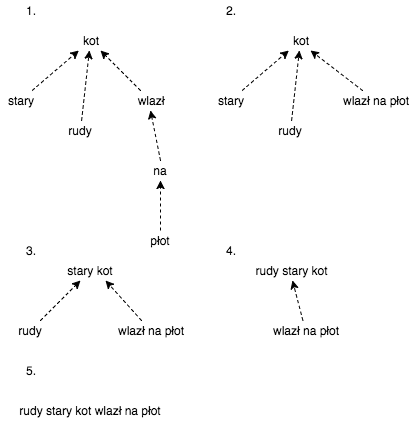
\includegraphics[width=0.5\textwidth]{staryrudykot}
		\caption{Przykład}
	\end{center}
\end{figure}
	
\section{Evaluation} 

\begin{table}[h]
 \begin{center}
\begin{tabular}{|l|l|}

      \hline
      %Level&Tools\\
      %\hline\hline
      Model & Score\\
      \hline
      LSTM &70,70\%\\
      \hline
      Lemmatized CRF & 75,63\%\\
      \hline
      Child-Sum Tree-LSTM &  77,69\%\\
      \hline
      Sequential-Child-Combination Tree-LSTM & 78,56\%\\
      \hline
      Lemmatized Child-Sum Tree-LSTM & 78,90\%\\
      \hline
      Lemmatized Sequential-Child-Combination Tree-LSTM & \textbf{79,89\%} \\
      \hline
\end{tabular}
\caption{Sentiment classification accuracy on the PolEval test set.}
\label{tab:evaluation}
 \end{center}
\end{table}



\section{Conclusions and future work}


\section{Availability}

The source code of the tagger described in this paper, together with the trained models, datasets, tagset translations and other resources such as the NCP Brown clusters are publicly available at \url{https://gitlab.com/piotr.pezik/apt_pl}.

%\nocite{*}

\bibliographystyle{ltc05}
\bibliography{sal} 

\end{document}

